\documentclass[
a4paper,
oneside,
10pt,
fleqn,
headsepline,
toc=listofnumbered, 
bibliography=totocnumbered]{scrartcl}

% deutsche Trennmuster etc.
\usepackage[T1]{fontenc}
\usepackage[utf8]{inputenc}
\usepackage[english, ngerman]{babel} % \selectlanguage{english} if  needed
\usepackage{lmodern} % use modern latin fonts

% Custom commands
\newcommand{\AUTHOR}{Michael Wieland}
\newcommand{\SECONDAUTHOR}{Fabian Hauser}
\newcommand{\INSTITUTE}{Hochschule für Technik Rapperswil}

% Jede Überschrift 1 auf neuer Seite
\let\stdsection\section
\renewcommand\section{\clearpage\stdsection}

% Multiple Authors
\usepackage{authblk}

% Include external pdf
\usepackage{pdfpages}

% Layout / Seitenränder
\usepackage{geometry}

% Inhaltsverzeichnis
\usepackage{makeidx} 
\makeindex

\usepackage{url}
\usepackage[pdfborder={0 0 0}]{hyperref}
\usepackage[all]{hypcap}
\usepackage{hyperxmp} % for license metadata

% Mathematik
\usepackage{amsmath}
\usepackage{amssymb}
\usepackage{amsfonts}
\usepackage{enumitem}

% Images
\usepackage{graphicx}
\graphicspath{{images/}} % default paths

% Boxes
\usepackage{fancybox}

%Tables
\usepackage{tabu}
\usepackage{booktabs} % toprule, midrule, bottomrule
\usepackage{array} % for matrix tables

% Multi Columns
\usepackage{multicol}

% Header and footer
\usepackage{scrlayer-scrpage}
\setkomafont{pagehead}{\normalfont}
\setkomafont{pagefoot}{\normalfont}
\automark*{section}
\clearpairofpagestyles
\ihead{\headmark}
\ohead{\TITLE}
\cfoot{\pagemark}

% Pseudocode
\usepackage{algorithm}
\usepackage{algorithmic}

% Code Listings
\usepackage{listings}
\usepackage{color}
\usepackage{beramono}

\definecolor{DarkPurple}{rgb}{0.4, 0.1, 0.4}
\definecolor{DarkCyan}{rgb}{0.0, 0.5, 0.4}
\definecolor{LightLime}{rgb}{0.3, 0.5, 0.4}
\definecolor{Blue}{rgb}{0.0, 0.0, 1.0}

\lstdefinestyle{eclipse-style}{
	language=Java,  
	columns=flexible,
	showstringspaces=false,     
	basicstyle=\footnotesize\ttfamily, 
	keywordstyle=\bfseries\color{DarkPurple},
	commentstyle=\color{LightLime},
	stringstyle=\color{Blue}, 
	escapeinside={£}{£}, % latex scope within code      
	morekeywords={length},
	numbers=left,
	numberstyle=\tiny\color{black},
	frame=single,
}
\lstset{style=eclipse-style}


% Theorems \begin{mytheo}{title}{label}
\usepackage{tcolorbox}
\tcbuselibrary{theorems}
\newtcbtheorem[number within=section]{definiton}{Definition}%
{fonttitle=\bfseries}{def}
\newtcbtheorem[number within=section]{remember}{Merke}%
{fonttitle=\bfseries}{rem}
\newtcbtheorem[number within=section]{hint}{Hinweis}%
{fonttitle=\bfseries}{hnt}

% Dokumentinformationen
\newcommand{\SUBJECT}{Report}
\newcommand{\TITLE}{Cloud Infrastructre Lab 1}

\begin{document}
	
% Front page
\title{\TITLE}
\subject{\SUBJECT}
\author{\SECONDAUTHOR}
\author{\AUTHOR}
\affil{\INSTITUTE}
\date{\today}
\maketitle

% Table of contents
\tableofcontents


% E-Mail to beat.stettler@ins.hsr.ch bis Donnerstag 23:59

%TODO: Übersicht logische topologie erstellen
%TODO: IP Adressplan erstellen
%TODO: Layer 2 und Layer 3 Protokolle angeben

%TODO: Verify and proof problems with measured date
%TODO: Empfehlungen für Anpassungen am Netzwerk
%TODO: Kostenvoranschlag für das Beheben der Fehler. Lösung mit dem kleinsten Einfluss auf das Produktive System und geringste Kosten


\section{Informationsbeschaffung}
In einem ersten Schritt wurden sämtliche Konfigurationen mit dem Tool Tftpd64 von den Router und Switches kopiert. Diese wurden dann in einem nächsten Schritt auf Fehlkonfigurationen analysiert. Dabei gingen wir nach folgendem Schema vor:

\begin{enumerate}
	\item Übersicht verschaffen. 
	\item Kopieren aller benötigten Konfigurationen
	\item Ordnen und Analysieren der Konfiguration. Was ist überhaupt vorhanden?
	\item Prüfen auf ''Common Mistakes'' mit besonderem Augenmerk auf die Layer 2 (VLAN, STP) und Layer 3 Protokolle (OSPF)
	\item Auswerten der gefunden Fehler
	\item Feedback und Lösungsvorschläge
\end{enumerate}

\subsection{Tools}
Für die Analyse wurden folgende Tools verwendet
\begin{enumerate}
	\item Tftpd64 um Konfigurationen zu dumpen
	\item jPerf um den Durchsatz zu messen
	\item Putty für die Telnet und Serielle Verbindung zu den Router und Switches
\end{enumerate}

\subsection{Terminologie}
Damit die Namen mehr an Bedeutung gewinnen, sollen folgend einige Abkürzungen nach besten Wissen ausgeschrieben werden.
\begin{multicols}{2}
\begin{description}
	\item[HQ] Head Quarter
	\item[BR] Branch
	\item[DS] Distribution Switch
	\item[CS] Core Switch
	\item[WER] WAN Exchange Router
	\item[IER] Internet Exchange Router
	\item[FRR] FrameRelayRouter
\end{description}
\end{multicols}


\subsection{Konfiguration kopieren}
Für jedes Geräte wurden die Outputs der folgenden Befehle auf die lokalen Notebooks kopiert. Alle Konfiguration sind im Anhang \ref{appendix:configurations} zu finden:
\begin{lstlisting}[language=bash]
copy run tftp und dann [your local ip addr]
show ip interface brief
show cdp neighbors
show interface status
show interface trunk
show vlan
show ip route
show spanning
\end{lstlisting}

\subsection{Analyse des Konfigurationen}
Folgende Tabellen dienen als Erweiterung zu den graphischen Schemas.
\subsection{DHCP}
\begin{table}[h]
	\centering
	\begin{tabu} to \linewidth {l l X}
		\toprule 
		DHCP Pool & Beschreibung & Bemerkung \\
		\midrule
		172.16.1.0/24 & HR &  \\
		172.16.2.0/24 & ENGINEERING &  \\
		172.16.3.0/24 & PRODUCTION &  \\
		172.16.4.0/24 & FINANCE &  \\
		172.16.16.0/24 & IT & DHCP exlude 172.16.16.1, 172.16.16.10 172.16.16.12 \\
		172.16.17.0/24 & SERVER & DHCP exclude 172.16.17.1, 172.16.17.10 172.16.17.12 \\
		172.16.18.0/24 & MARKETING & DHCP exclude 172.16.18.250, 172.16.18.254, 172.16.18.10 172.16.18.12  \\
		172.16.19.0/24 & SALES & DHCP exclude 172.16.19.250, 172.16.19.254, 172.16.19.10 172.16.19.12 \\
		172.16.103.0/24 & Branch 2 & DHCP exlude 172.16.103.1, 172.16.103.10, 172.16.103.12 \\
		\bottomrule 
	\end{tabu} 
	\caption{DHCP Pools}
\end{table}

\subsection{VLAN}
IEEE 802.1Q = Paketbasierte tagged VLAN's
\begin{table}[h]
	\centering
	\begin{tabu} to \linewidth {l l l}
		\toprule 
		VLAN & Name & Bedeutung \\
		\midrule
		VLAN 10 & HR & Personalabteilung \\
		VLAN 11 & IT & IT Abteilung \\
		VLAN 99 & MGMT & Management\\
		VLAN 100 & STAFF & Mitarbeiter\\
		VLAN 150 & IWAS & ???\\
		VLAN 200 & STUDENTS & Studenten\\
		\bottomrule 
	\end{tabu} 
	\caption{VLAN's}
\end{table}

\begin{table}[h]
	\centering
	\begin{tabu} to \linewidth {l l l}
		\toprule 
		VLAN & Subnetz & Bemerkung \\
		\midrule
		VLAN1 & 172.16.103.0/24 & \\
		VLAN10 & 172.16.1.0/24 & \\
		VLAN11 & 172.16.2.0/24 & \\
		VLAN20 & no ip addr assigned & (router ospf) \\
		VLAN21 & 172.16.16.0/24 & (mtu-ignore) \\
		VLAN30 & 172.16.17.0/24 & \\
		VLAN40 & 172.16.18.0/24 & (standby) \\
		VLAN41 & 172.16.19.0/24 & (mtu ignore) \\
		VLAN100 & 172.16.20.0/24 & (mtu ignore) \\
		VLAN103 & 172.16.23.0/24 & \\
		\bottomrule 
	\end{tabu} 
	\caption{VLAN Subnetze}
\end{table}

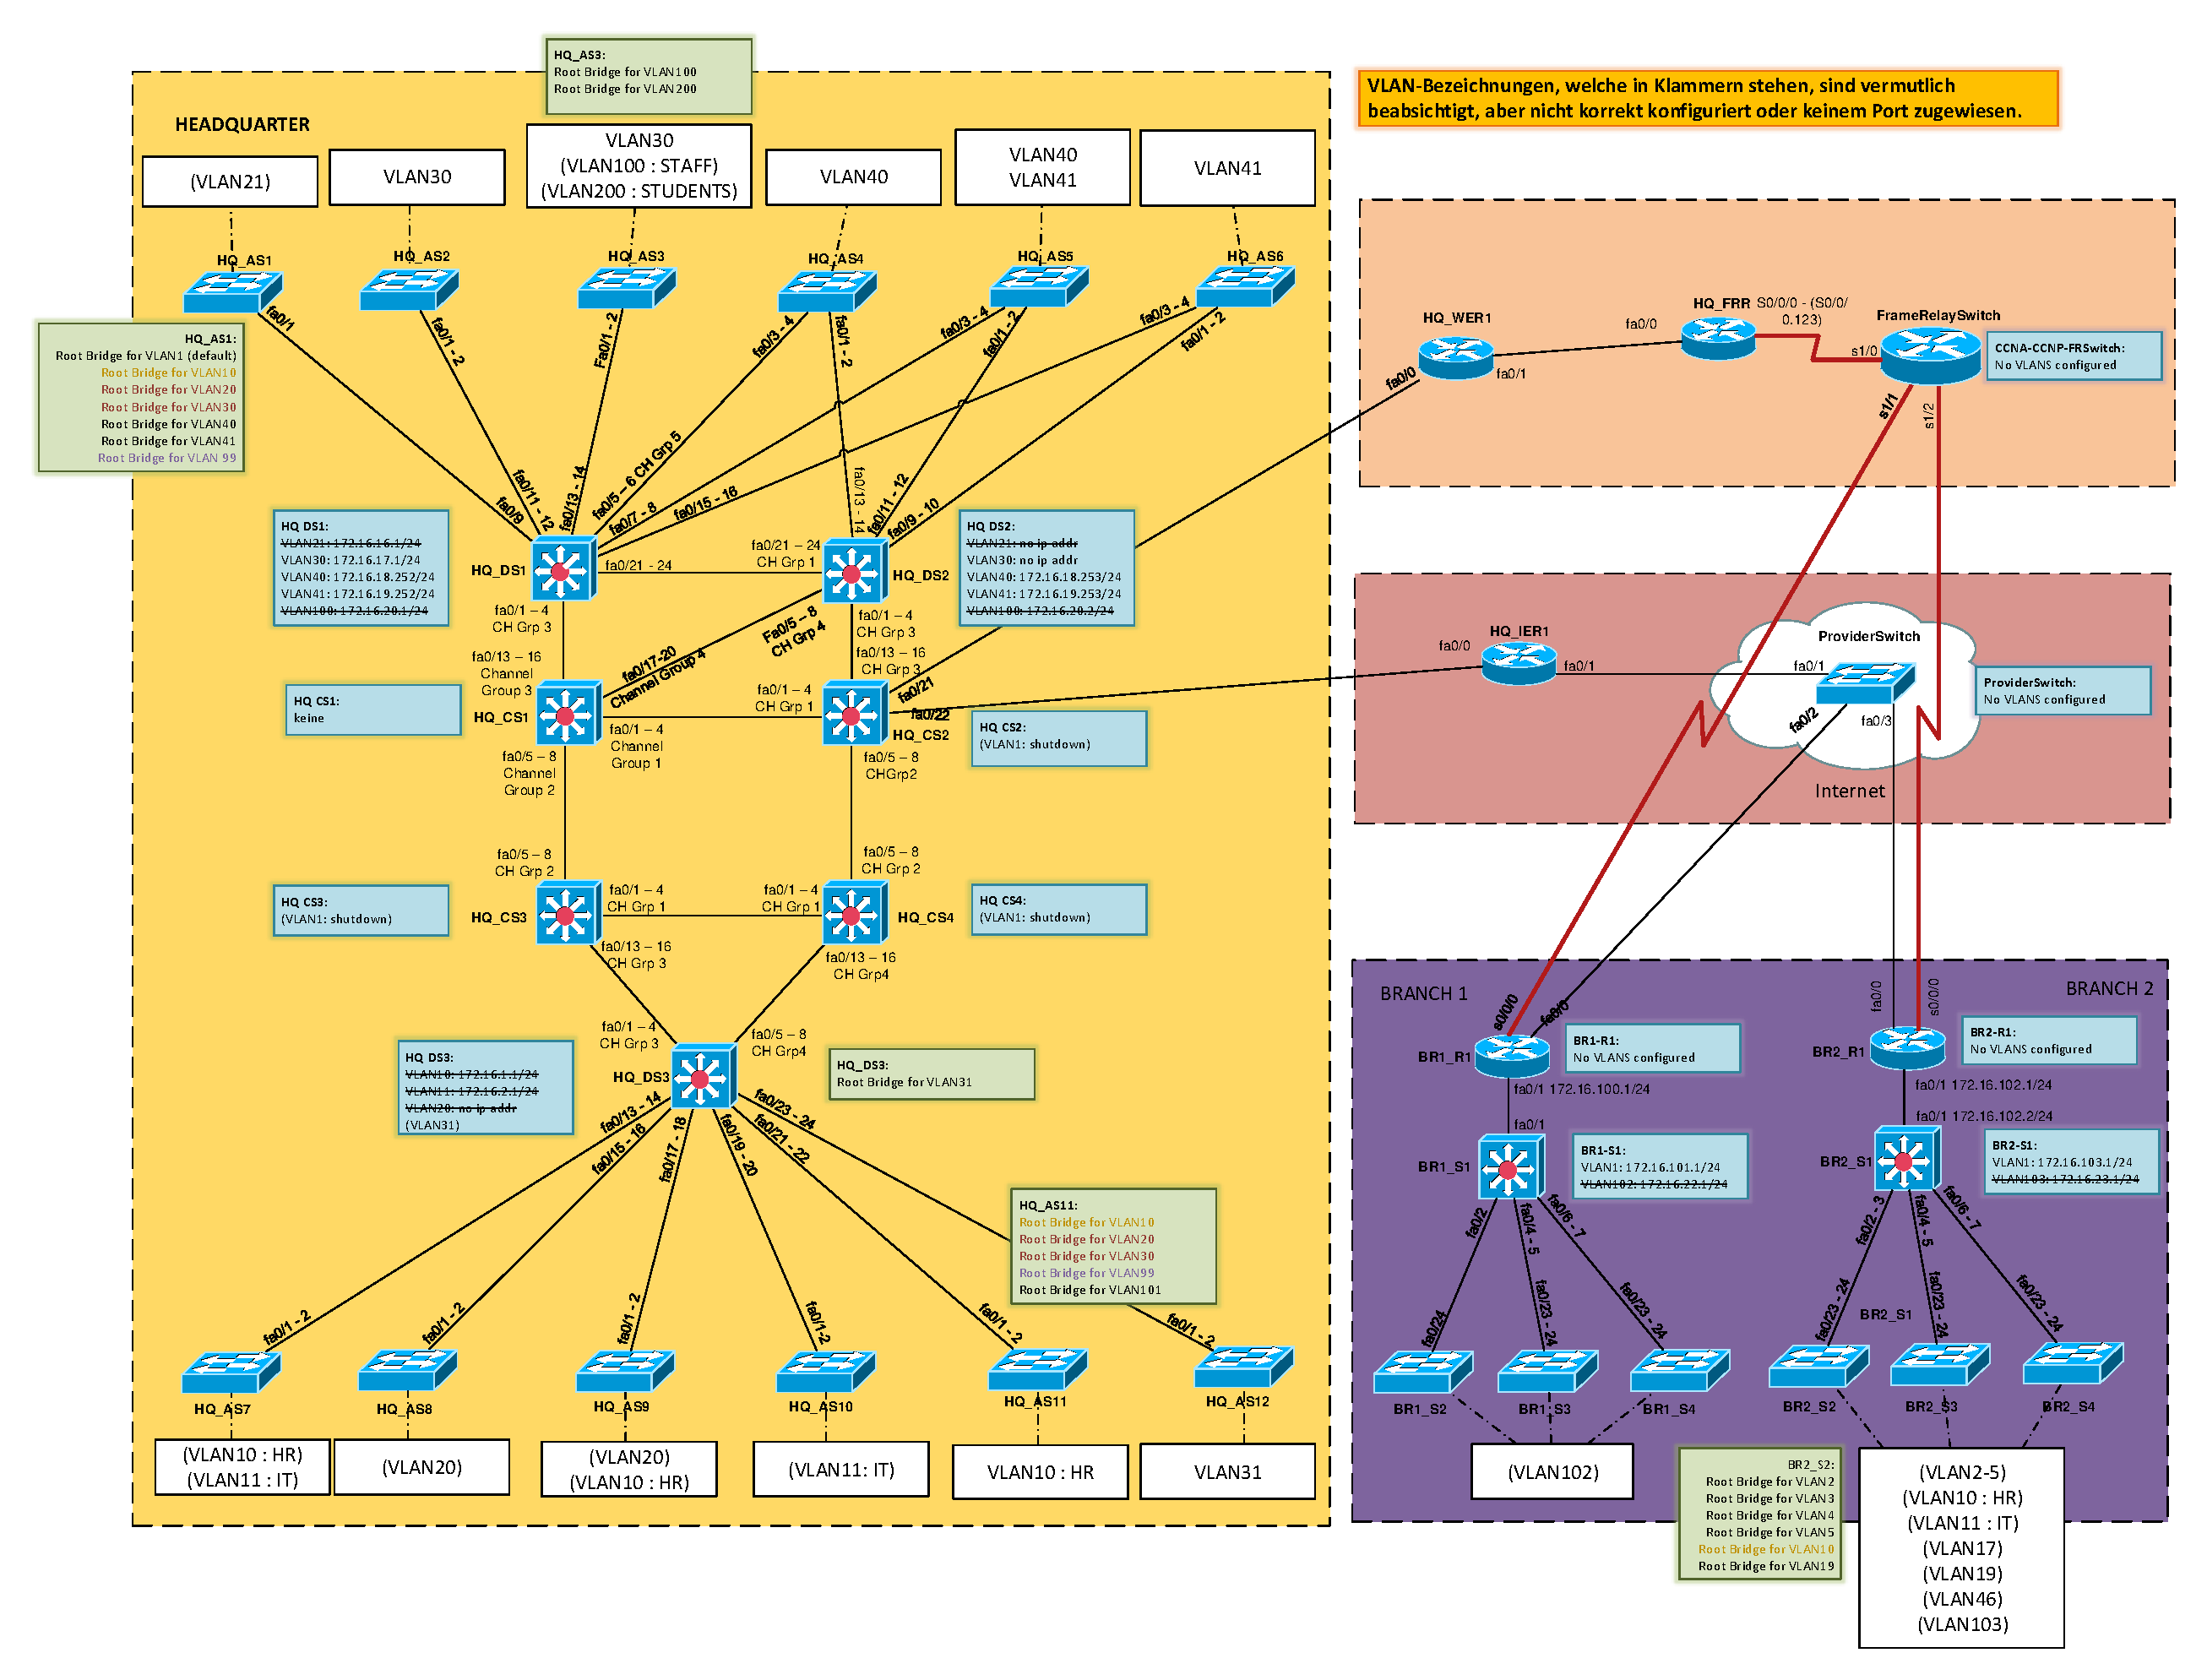
\includepdf[pages={1},landscape=true]{appendix/schemes/vlan.pdf}
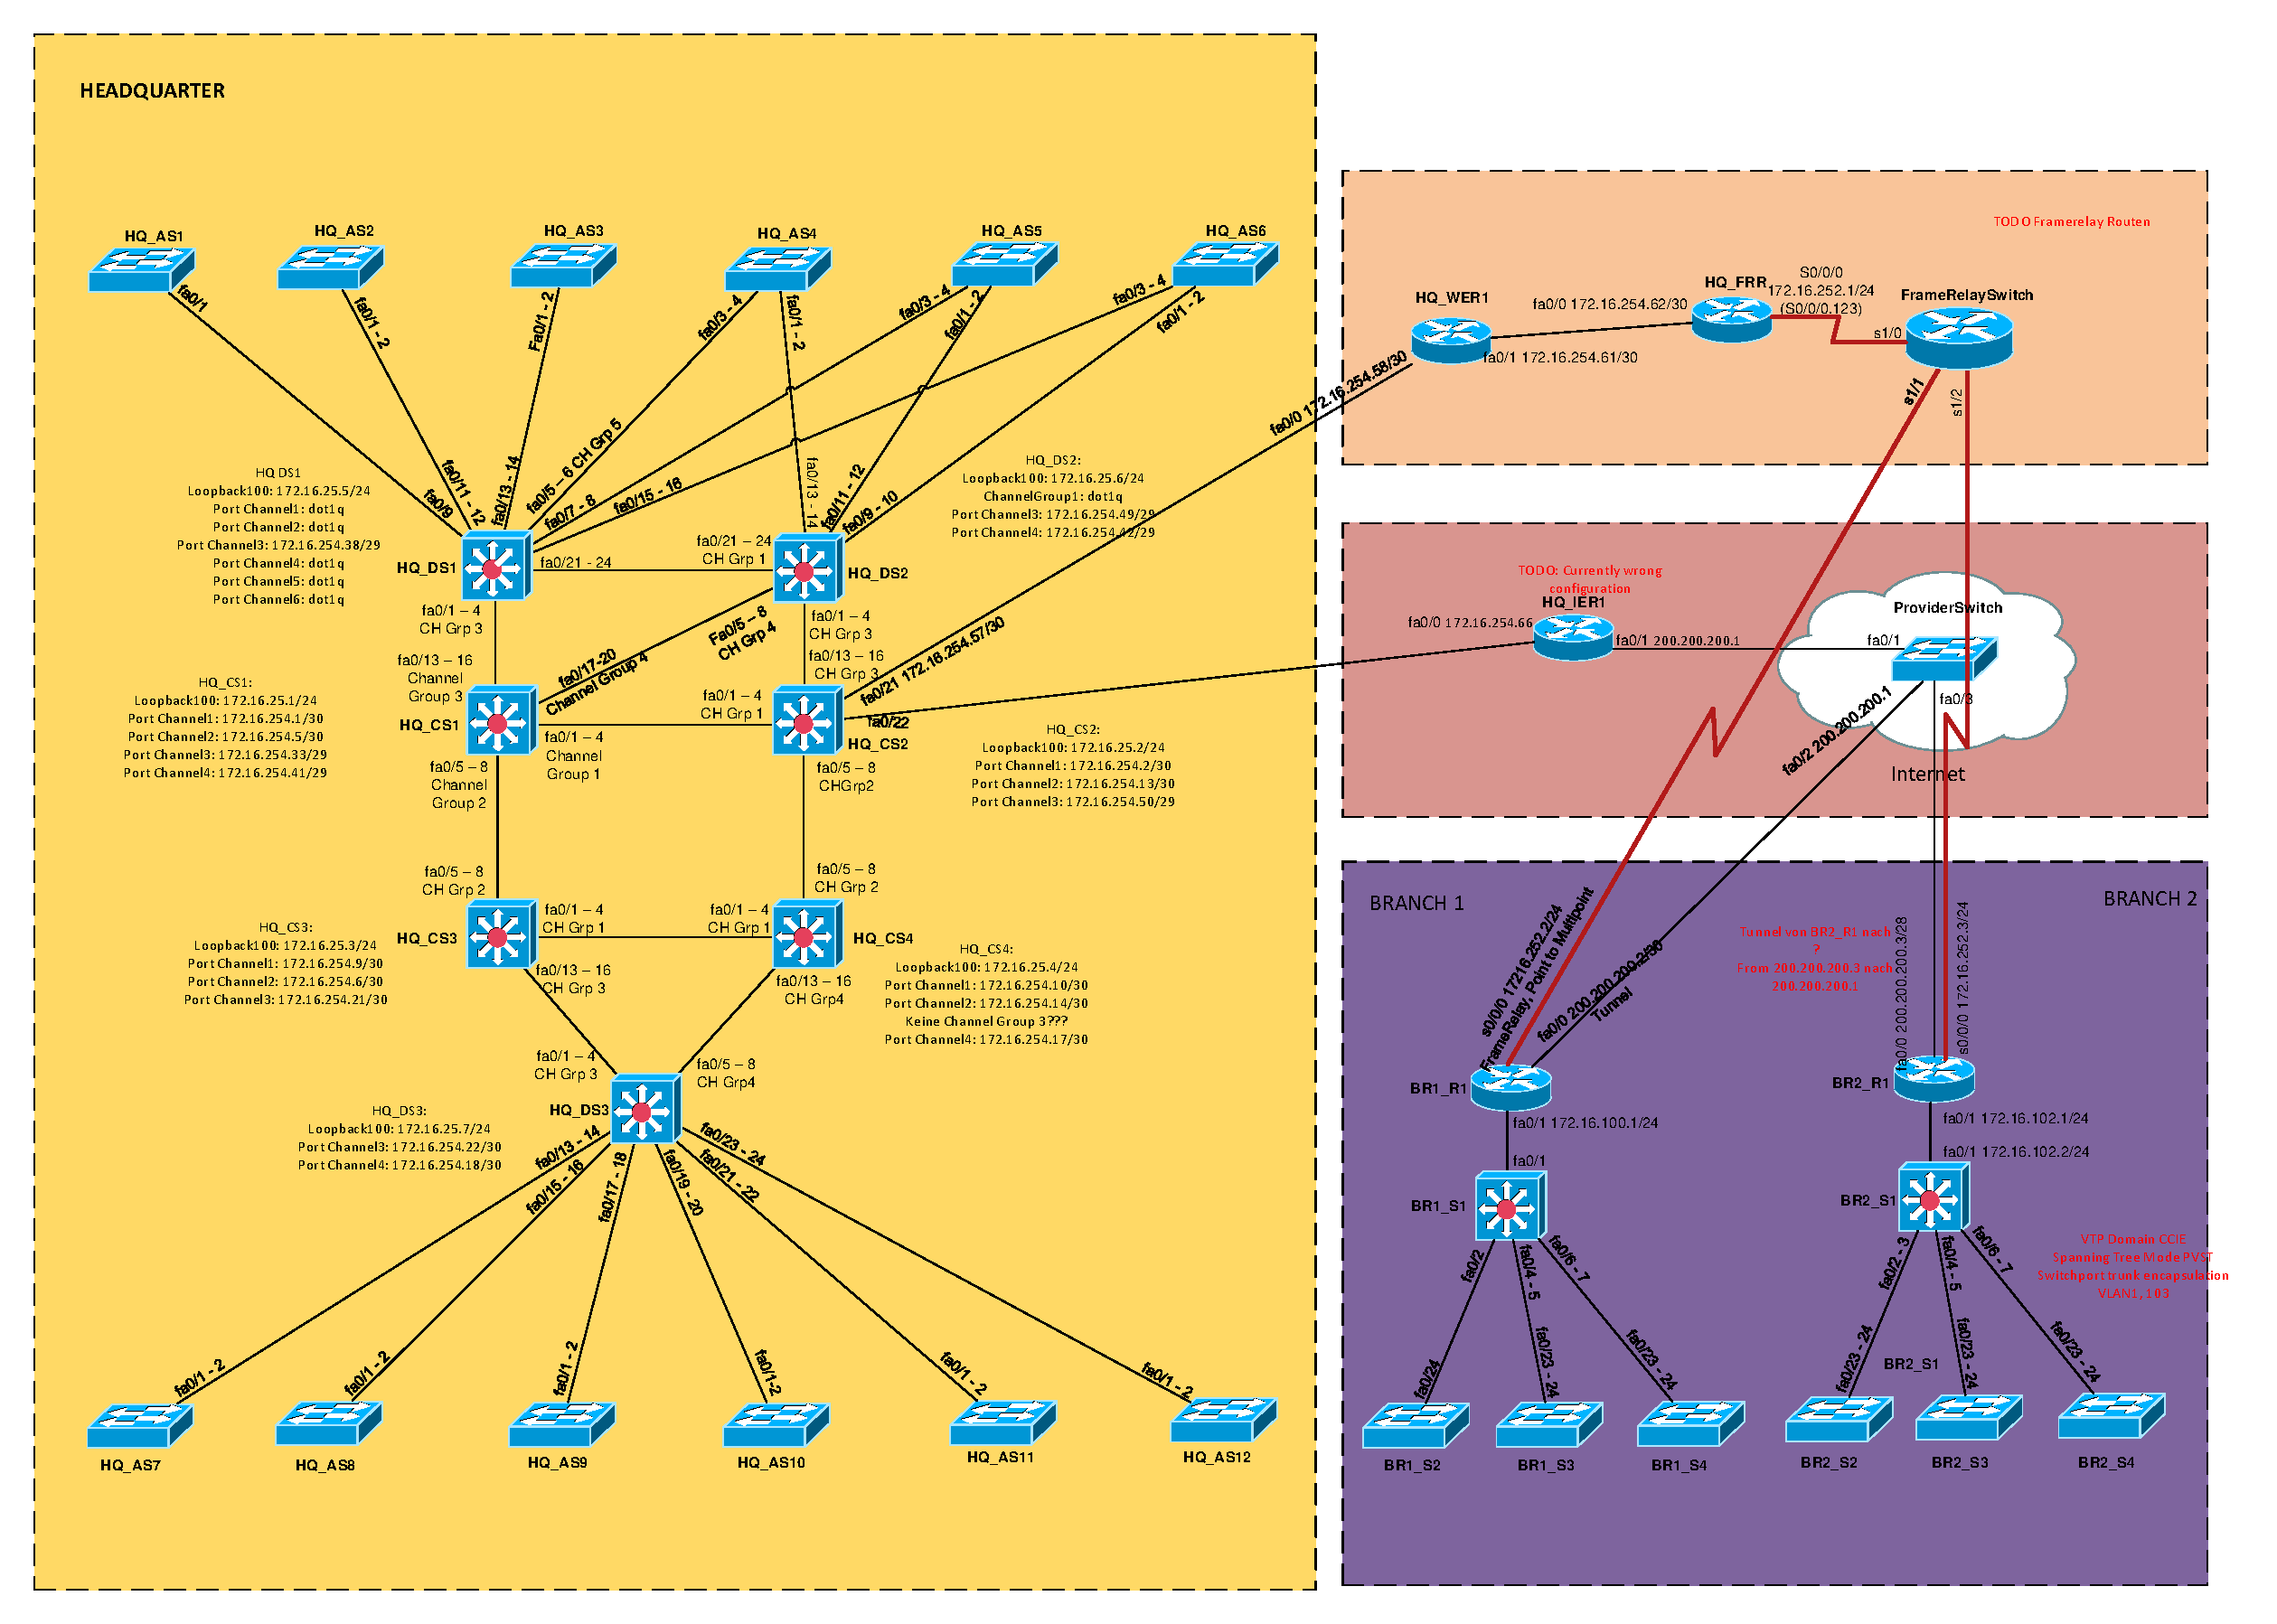
\includepdf[pages={1},landscape=true]{appendix/schemes/L1.pdf}

\section{Gefundene Fehler}

Unschön: Bei vertippern im Komando wird immer nache dem Nameserver gesucht.

\subsection{Layer 1}
Auf OSI Layer 1 wurden keine Fehler gefunden.

\subsection{Layer 2}
%TODO Auf CCNA-CCNP-FRSwitch ist CDP (Cisco ???) nicht aktiviert

\subsubsection{Design}
\begin{itemize}
	\item HQ\_CS2 bildet die einzige Verbindung zu den Branches. Es bildet somit einen Single Point of Failure
\end{itemize}

\subsubsection{Speed}
\begin{itemize}
	\item Die Port Channel Group 4 beim HQ\_CS1 ist auf Half Duplex 100Mbit/s eingestellt.
	\item Die Port Channel Group 2 bei HQ\_CS2 ist auf 10Mbit/s eingestellt. 
\end{itemize}

\subsubsection{Spanning Tree}

\subsubsection{VLAN}
\begin{itemize}
	\item VLAN1 auf HQ\_AS1 ist Administratively Down
	\item Nur Fa0/2, Gi0/1, Gi0/2 sind auf HQ\_AS1 für VLAN1 konfiguriert, andere Ifs sind nicht eingerichtet
	\item
\end{itemize}

\subsection{Layer 3}

\subsubsection{Routen}

\subsection{OSPF}


\section{Messungen}
\subsection{Traceroute}
Alle Durchgeführten Traceroute Messungen sind im Anhang \ref{appendix:measures} zu finden.

% TODO add folgerungen


%TODO Ist ein Port mit langsamem Durchsatz konfiguriert?

\subsection{jPerf}




\section{Empfehlungen}
Aufgrund der vorangehenden Erkenntnissen empfehlen wir, an folgenden Punkten anzusetzen:
%TODO add recommedations
\begin{enumerate}
	\item Alle 10 und 100Mbit/s Leitung auf den maximal physisch möglichen Durchsatz aufschrauben.
\end{enumerate}

\subsection{Kostenvoranschlag}
Für die Umsetzung unserer Empfehlungen würden folgende Kosten anfallen.
\begin{table}[h]
	\centering
	\begin{tabu} to \linewidth {l l l l}
		\toprule 
		Beschreibung & Zeitaufwand in h  & Stundenansatz in CHF & Total \\
		\midrule
		&&& \\
		\textbf{Total} & & & \underline{\underline{1 Million}} \\
		\bottomrule 
	\end{tabu} 
	\caption{Kostenvoranschlag}
\end{table}

\appendix

\section{Konfigurationen}
\label{appendix:configurations}

\subsection{BR1-R1}
\subsubsection{Running Configuration}
\lstinputlisting{appendix/config/br1-r1/br1-r1-config.txt}

\subsubsection{IP Interfaces}
\lstinputlisting{appendix/config/br1-r1/br1-r1-interface.txt}

\subsubsection{Interface Status}
\lstinputlisting{appendix/config/br1-r1/br1-r1-status.txt}

\subsubsection{Neighbors}
\lstinputlisting{appendix/config/br1-r1/br1-r1-neighbors.txt}

\subsection{BR2-R1}
\subsubsection{Running Configuration}
\lstinputlisting{appendix/config/br2-r1/br2-ri-config.txt}

\subsubsection{IP Interfaces}
\lstinputlisting{appendix/config/br2-r1/br2-ri-interface.txt}

\subsubsection{Interface Status}
\lstinputlisting{appendix/config/br2-r1/br2-ri-status.txt}

\subsubsection{Neighbors}
\lstinputlisting{appendix/config/br2-r1/br2-ri-neighbors.txt}

\subsection{BR2-S1}
\subsubsection{Running Configuration}
\lstinputlisting{appendix/config/br2-s1/br2-s1-config.txt}

\subsubsection{IP Interfaces}
\lstinputlisting{appendix/config/br2-s1/br2-s1-interface.txt}

\subsubsection{Interface Status}
\lstinputlisting{appendix/config/br2-s1/br2-s1-status.txt}

\subsubsection{Neighbors}
\lstinputlisting{appendix/config/br2-s1/br2-s1-neighbors.txt}

\subsection{CCNA-CCNP-FRSwitch}
\subsubsection{Running Configuration}
\lstinputlisting{appendix/config/framerelayswitch/framerelayswitch-config.txt}

\subsubsection{IP Interfaces}
\lstinputlisting{appendix/config/framerelayswitch/framerelayswitch-interface.txt}

\subsubsection{Interface Status}
\lstinputlisting{appendix/config/framerelayswitch/framerelayswitch-status.txt}

\subsubsection{Neighbors}
\lstinputlisting{appendix/config/framerelayswitch/framerelayswitch-neighbors.txt}

\subsection{HQ FrameRelay Router (HQ-FRR)}
\subsubsection{Running Configuration}
\lstinputlisting{appendix/config/hq-frr/hq-frr-config.txt}

\subsubsection{IP Interfaces}
\lstinputlisting{appendix/config/hq-frr/hq-frr-interface.txt}

\subsubsection{Interface Status}
\lstinputlisting{appendix/config/hq-frr/hq-frr-status.txt}

\subsubsection{Neighbors}
\lstinputlisting{appendix/config/hq-frr/hq-frr-neighbors.txt}

\subsection{HQ-IER1}
\subsubsection{Running Configuration}
\lstinputlisting{appendix/config/hq-ier1/hq-ier1-config.txt}

\subsubsection{IP Interfaces}
\lstinputlisting{appendix/config/hq-ier1/hq-ier1-interface.txt}

\subsubsection{Interface Status}
\lstinputlisting{appendix/config/hq-ier1/hq-ier1-status.txt}

\subsubsection{Neighbors}
\lstinputlisting{appendix/config/hq-ier1/hq-ier1-neighbors.txt}

\subsection{HQ-WER1}
\subsubsection{Running Configuration}
\lstinputlisting{appendix/config/hq-wer1/hq-wer1-config.txt}

\subsubsection{IP Interfaces}
\lstinputlisting{appendix/config/hq-wer1/hq-wer1-interface.txt}

\subsubsection{Interface Status}
\lstinputlisting{appendix/config/hq-wer1/hq-wer1-status.txt}

\subsubsection{Neighbors}
\lstinputlisting{appendix/config/hq-wer1/hq-wer1-neighbors.txt}

\subsection{HQ CS1}
\subsubsection{Running Configuration}
\lstinputlisting{appendix/config/hq-cs1/hq-cs1-config.txt}

\subsubsection{IP Interfaces}
\lstinputlisting{appendix/config/hq-cs1/hq-cs1-interface.txt}

\subsubsection{Interface Status}
\lstinputlisting{appendix/config/hq-cs1/hq-cs1-status.txt}

\subsubsection{Neighbors}
\lstinputlisting{appendix/config/hq-cs1/hq-cs1-neighbors.txt}

\subsection{HQ CS2}
\subsubsection{Running Configuration}
\lstinputlisting{appendix/config/hq-cs2/hq-cs2-config.txt}

\subsubsection{IP Interfaces}
\lstinputlisting{appendix/config/hq-cs2/hq-cs2-interface.txt}

\subsubsection{Interface Status}
\lstinputlisting{appendix/config/hq-cs2/hq-cs2-status.txt}

\subsubsection{Neighbors}
\lstinputlisting{appendix/config/hq-cs2/hq-cs2-neighbors.txt}

\subsection{HQ CS3}
\subsubsection{Running Configuration}
\lstinputlisting{appendix/config/hq-cs3/hq-cs3-config.txt}

\subsubsection{IP Interfaces}
\lstinputlisting{appendix/config/hq-cs3/hq-cs3-interface.txt}

\subsubsection{Interface Status}
\lstinputlisting{appendix/config/hq-cs3/hq-cs3-status.txt}

\subsubsection{Neighbors}
\lstinputlisting{appendix/config/hq-cs3/hq-cs3-neighbors.txt}

\subsection{HQ CS4}
\subsubsection{Running Configuration}
\lstinputlisting{appendix/config/hq-cs4/hq-cs4-config.txt}

\subsubsection{IP Interfaces}
\lstinputlisting{appendix/config/hq-cs4/hq-cs4-interface.txt}

\subsubsection{Interface Status}
\lstinputlisting{appendix/config/hq-cs4/hq-cs4-status.txt}

\subsubsection{Neighbors}
\lstinputlisting{appendix/config/hq-cs4/hq-cs4-neighbors.txt}

\subsection{HQ DS1}
\subsubsection{Running Configuration}
\lstinputlisting{appendix/config/hq-ds1/hq-ds1-config.txt}

\subsubsection{IP Interfaces}
\lstinputlisting{appendix/config/hq-ds1/hq-ds1-interface.txt}

\subsubsection{Interface Status}
\lstinputlisting{appendix/config/hq-ds1/hq-ds1-status.txt}

\subsubsection{Neighbors}
\lstinputlisting{appendix/config/hq-ds1/hq-ds1-neighbors.txt}

\subsection{HQ DS2}
\subsubsection{Running Configuration}
\lstinputlisting{appendix/config/hq-ds2/hq-ds2-config.txt}

\subsubsection{IP Interfaces}
\lstinputlisting{appendix/config/hq-ds2/hq-ds2-interface.txt}

\subsubsection{Interface Status}
\lstinputlisting{appendix/config/hq-ds2/hq-ds2-status.txt}

\subsubsection{Neighbors}
\lstinputlisting{appendix/config/hq-ds2/hq-ds2-neighbors.txt}

\subsection{HQ DS3}
\subsubsection{Running Configuration}
\lstinputlisting{appendix/config/hq-ds3/hq-ds3-config.txt}

\subsubsection{IP Interfaces}
\lstinputlisting{appendix/config/hq-ds3/hq-ds3-interface.txt}

\subsubsection{Interface Status}
\lstinputlisting{appendix/config/hq-ds3/hq-ds3-status.txt}

\subsubsection{Neighbors}
\lstinputlisting{appendix/config/hq-ds3/hq-ds3-neighbors.txt}


\section{Messungen}
\label{appendix:measures}
\subsection{Von X nach Y}
\lstinputlisting{appendix/config/br2-r1/br2-ri-config.txt}

% Code Listings
% \lstlistoflistings

% List of figures
% \listoffigures

% List of tables
% \listoftables

% Bibliography
% \bibliographystyle{plain} 
% \bibliography{literatur}

\end{document}